\chapter{Implementation}
% ==Structure== %
Because the work this project is based on used double precision data types this is done here as well, to make sure
errors are not due to insufficient accuracy. A switch to single precision data types was left as a question to be
evaluated based on results from testing.

In contrast to the previous work however, this simulation is done in 3D, adding realism at the cost of accuracy. Adding
an additional dimension increases the number of cells by resolution in that dimension times the number of cells in the
plane. Because the memory usage and algorithm complexity increases, the resolution of each dimension will be limited.
A 3D grid of $256^3$ contains the same number of cells as a 2D grid at $4096^2$.

% % =Kernels= %
\section{Kernels}
A description of the kernels follow.

% % determineChargesFromPotential %
\subsection{determineChargesFromPotential}
The kernel determining the charge density of the mesh from particle charges. The contribution of a particle to each
vertex of its resident cell is found using trilinear interpolation, illustrated in fig. \ref{fig:trilinear}. The
distribution of a particle charge $\rho_p$ is as follows:
\begin{align*}
                \rho(i, j, k) \quad &+=\quad \frac{\rho_p }{ (h_x \cdot h_y \cdot h_z)} \cdot (h_x-a) \cdot (h_y-b) \cdot (h_z-c)\\
            \rho(i+1, j, k) \quad &+=\quad \frac {\rho_p }{ (h_x \cdot h_y \cdot h_z)} \cdot (h_x-a) \cdot b \cdot (h_z-c)         \\
            \rho(i, j+1, k) \quad &+=\quad \frac {\rho_p }{ (h_x \cdot h_y \cdot h_z)} \cdot a \cdot (h_y-b) \cdot (h_z-c)         \\
       \rho(i+1, j+1, k) \quad &+=\quad \frac{\rho_p }{ (h_x \cdot h_y \cdot h_z)} \cdot a \cdot b \cdot (h_z-c)                   \\
           \rho(i, j, k+1) \quad &+=\quad \frac{\rho_p }{ (h_x \cdot h_y \cdot h_z)} \cdot (h_x-a) \cdot (h_y-b) \cdot c         \\
      \rho(i+1, j, k+1) \quad &+= \quad \frac{\rho_p }{ (h_x \cdot h_y \cdot h_z)} \cdot (h_x-a) \cdot b \cdot c                   \\
      \rho(i, j+1, k+1) \quad &+= \quad \frac{\rho_p }{ (h_x \cdot h_y \cdot h_z)} \cdot a \cdot (h_y-b) \cdot c                   \\
 \rho(i+1, j+1, k+1) \quad &+= \quad \frac{\rho_p }{ (h_x \cdot h_y \cdot h_z)} \cdot a \cdot b \cdot c
\end{align*}
As can be seen, the contribution for a vertex is proportional to its distance to the particle compared to the other
vertices, the closest one receives the most charge and all contributions sums to $\rho_p$. Visualized in figure \ref{fig:trilinear},
dividing the cells along the interpolation lines, the contribution of a vertex is proportional to the volume of the
opposite sub-prism. We can see that the variable terms of the equations above give the volume, for instance
$\rho(i+1, j+1, k+1)$ has the term $a\cdot b\cdot c$ which is the volume of the prism in the opposite corner.

The kernel as is does not use shared memory to reduce memory latency, and it relies on slow atomic operations to avoid
write conflicts.

\begin{figure}
	\centering
	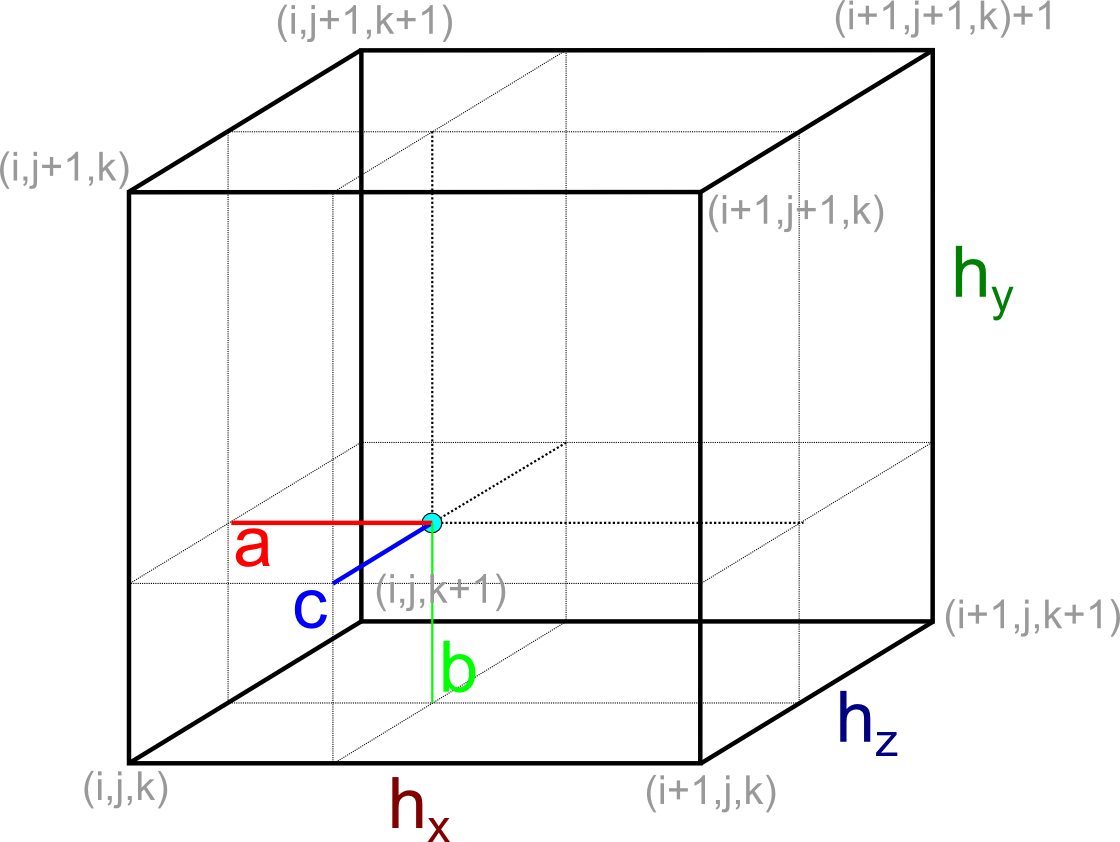
\includegraphics[width=0.8\textwidth]{figure/trilinear}
	\caption{Trilinear interpolation of particles with mesh vertices.}
	\label{fig:trilinear}
\end{figure}

% % electricFieldFromPotential %
\subsection{electricFieldFromPotential}
The electric field strength at a point is approximated as the difference in potential between it's neighbors, measured
separately in each dimension.
\begin{align*}
	E_x &= \Phi_{i+1} - \Phi_{i-1}\\
	E_y &= \Phi_{j+1} - \Phi_{j-1}\\
	E_z &= \Phi_{k+1} - \Phi_{k-1}
\end{align*}
The electric field is therefore stored as a vector at each point in the grid (array of structures).

\paragraph{electricFieldAtPoint} is a device helper function for doing trilinear interpolation of the electric field strength at some floating point
position. Similarly to the charge density calculations, field strength at a position is accumulated from cell vertices,
with contribution from each one proportional to the distance to it.

% % updateParticles %
\subsection{updateParticles}
\begin{lstlisting}
	ax = p.electricfield.x * cfg.charge_by_mass;
	prev = (1 - cfg.drag * cfg.ts);
	p.velocity.x = p.velocity.x * prev + ax * cfg.ts;
	p.position.x += p.velocity.x * cfg.ts;
\end{lstlisting}
The particle update kernel first finds the field electrical field strength at the particle's position using the helper
function electricFieldAtPoint, and then the acceleration using $a_p=\frac{F_e}{m_p} = \frac{E \cdot q_p}{m_p}$. Velocity and position
is updated through a leap frog method, where there is a $^{\Delta t}\!/_2$ delay between velocity and position updates.
$$ v^{n+ ^1\!/_2 } = v^{n+ ^1\!/_2 } + a^n \cdot \Delta t $$
$$ p^{n+1} = p^n + v^n \cdot \Delta t $$
The result is that a position update uses a velocity value that lies between the two points in time, an "average" value,
and similarly for velocity updates.


% =cuFFT= %
\section{cuFFT}
The FFT-based solver uses the cuFFT library, and this section will therefore focus on usage rather than implementation.

\subsection{FFT setup}
To run an FFT a plan has to be set up first, and stored using a cufftHandle. For single transforms with simple data
layouts the cufftPlan\#d() functions provide a simple interface for 1D, 2D and 3D transforms, while more complex setups
may need to use cufftPlanMany(). This function allows input and output  to be batched and strided data. All plans
specify the data types of the transform with options of \emph{real-to-complex}, \emph{complex-to-real}(implicitly an
inverse transform), or \emph{complex-to-complex}, and single or double precision. R stands for real, C for complex,
while D and Z are the same only for double precision.
\begin{lstlisting}
//cufftPlanMany signature
cufftResult cufftPlanMany(
	cufftHandle *plan,// Pointer to the plan
	int rank,					// dimensionality, (1, 2 or 3)
	int *n,						// n[i] = size of dimension i
	int *inembed,			// Size of dimensions in storage
	int istride,			// Distance between elements in inner dimension
	int idist,				// Distance between first elements in a batch
	int *onembed,			// Same as the above but for output
	int ostride,			// ...
	int odist,				// ...
	cufftType type,		// real or complex, single or double precision
	int batch					// multiple transforms with one call
);
\end{lstlisting}

\subsection{FFT call}
After the plan has been created, the transform can be executed using cufftExecX2X(). X2X may be either R2C, C2R, C2C,
D2Z, Z2D, Z2Z and must match the type parameter of the plan. In addition to the plan generated using cufftPlanXX(),
pointers to input and output data must ge supplied. For C2C and Z2Z an additional direction parameter must be set. R2C
is implicitly forward, Z2D is implicitly inverse and so on.
\begin{lstlisting}
//cufftExecC2C signature
cufftResult cufftExecC2C(
	cufftHandle plan,			// Plan generated as above
	cufftComplex *idata,	// Input data pointer
	cufftComplex *odata,	// output data pointer
	int direction					// Direction (forward/inverse)
);
\end{lstlisting}
\begin{lstlisting}
// Example cufft procedure
cufftHandle plan, iplan;
cufftCreate(&plan);
cufftCreate(&iplan);
cufftPlanMany(plan, ...); // Paln the transforms
cufftPlanMany(iplan, ...);
cufftExecR2C(plan, ...); // Forward transform
// ...
// Do something in spectral domain.
// ...
cufftExecC2R(iplan, ...); // Inverse transform
\end{lstlisting}

% solve %
\paragraph{solve}
After the data has been transformed using cufft, solving the for the field is done by multiplying each value by
$^1\!/_{k^2} $, and then scaling by $ ^1\!/_{\epsilon_0} $ to get $\Phi$.

$$ \frac{1}{{\epsilon_0 \cdot \left(
	\left(\frac{(2\pi \cdot \text{i} }{ L_x}\right)^2 + \left(\frac{2\pi \cdot \text{j} }{ L_y}\right)^2 + \left(\frac{2\pi \cdot \text{k} }{ L_z}\right)^2
\right)}} $$

 In addition, we need to normalize the transformation, scaling the elements by the size of the data set, which is
 $N_x \cdot N_y \cdot N_z$. The resulting computation is then to multiply the value at (i, j, k) by
 $$ \frac{1}{{4\pi^2 \cdot \epsilon_0 \cdot N_x \cdot N_y \cdot N_z \cdot \left(\, ^{\text{i}^2}\!/_{L_x^2} +\, ^{\text{j}^2}\!/_{L_y^2} +\, ^{\text{k}^2}\!/_{L_z^2}\right)}} $$
\begin{lstlisting}
scale_factor = 1/(eps_0 * 4*pi*pi * n.x * n.y * n.z);

double scale = scale_factor /
			(i*i/(l.x*l.x) + j*j/(l.y*l.y) + k*k/(l.z*l.z));

//Complex number:
row[i].x *= scale;
row[i].y *= scale;
\end{lstlisting}

% =SOR= %
\section{SOR}
From Gauss's law we have
\begin{align*}
	\nabla^2\Phi =& \frac{\partial^2\Phi}{\partial x^2} + \frac{\partial^2\Phi}{\partial y^2} + \frac{\partial^2\Phi}{\partial z^2} = - \frac{\rho_f}{\epsilon_0}\\
\intertext{This is approximated using second order finite differences.}
	\nabla^2\Phi \approx& \frac{ \Phi_{i-1} + \Phi_{i+1} + \Phi_{j-1} + \Phi_{j+1} + \Phi_{k-1} + \Phi_{k+1} - 6\Phi_{i, j, k}}{h_x \cdot h_y \cdot h_z} = -\frac{\rho_{i, j, k}}{\epsilon_0}\\
\intertext{We solve for $\Phi_{i, j, k}$}
	\Phi_{i, j, k} =& \frac{\rho_{i, j, k}\cdot\frac{h_x h_y h_z}{\epsilon_0} + \Phi_{i-1} + \Phi_{i+1} + \Phi_{j-1} + \Phi_{j+1} + \Phi_{k-1} + \Phi_{k+1}}{6}\\
\intertext{Over-relaxed updates use}
	\Phi_{i, j, k}^{(n+1)} =& (\omega-1)\Phi_{i, j, k}^{(n)} + \omega\cdot\frac{\Phi_{i-1}^{(n)} + \Phi_{i+1}^{(n)} + \Phi_{j-1}^{(n)} + \Phi_{j+1}^{(n)} + \Phi_{k-1}^{(n)} + \Phi_{k+1}^{(n)}}{6}\\
	\Phi_{i, j, k}^{(n+1)} =& \Phi_{i, j, k}^{(n)} + \numberthis \label{eqn:sor-update}\\
	&\; \omega \cdot \left( \frac{\Phi_{i-1}^{(n)} + \Phi_{i+1}^{(n)} + \Phi_{j-1^{(n)}} + \Phi_{j+1^{(n)}} + \Phi_{k-1}^{(n)} + \Phi_{k+1}^{(n)}}{6}-\Phi_{i, j,k}^{(n)} \right) 
\end{align*}
The SOR solver builds on the red-black Jacobi method described in \ref{sec:red-black}, using over relaxation to speed up
convergence. While previous work\cite[sec.~3.3.3]{elster94}\cite[sec.~2.7.2]{larsgaard07} used five-point stencils in a 2D solver, a seven-point
stencil is used to account for the z dimension, this being a 3D solver. For this solver boundary values are set equal to
the center value ($\Phi_{i, j, k}$).

As is, the kernel is run a fixed number of times, rather than checking the error. Every iteration the kernel is run
twice, once each for red and black colored tiles, allowing in-place updates in parallel.

% SOR kernel %
\paragraph{SOR kernels}
An initSOR kernel is run first, saturating the \emph{Phi} array with the appropriate values,
$$ \Phi_{i, j, k} = \frac{\rho_{i, j, k}\cdot h_x h_y h_z}{6 \cdot \epsilon_0} $$

When the SOR kernel itself is called, the \emph{k} index is calculated as follows, in order to implement red-black
coloring:
$$k = 2 \cdot Idx.z + (i + j + flag) \% 2 $$
where flag is 0 or 1 depending on whether red or black tiles are updated. The update itself uses equation \ref{eqn:sor-update}:

\begin{lstlisting}
	tmp = (left + right + down + up + front + back)/6;
	Phi[i][j][k] = center + cfg.omega * (tmp - center);
\end{lstlisting}


% =Setup= %
\section{Setup}\label{sec:implementation-setup}
The implementation currently uses parameters set in a getConfig() function, rather than with preprocessor macros. While
this prevents the compiler from optimizing certain calculations it allows parameters to be read in at runtime,
functionality that existed in Elster's original implementation, which this one it intended to be a CUDA version of.
Parameters that can be set and their default values for testing are shown in section \ref{sec:testing-parameters}.

All device memory allocations except that for the particle array use pitched pointers to ensure data alignment, helping
ensure coalesced memory accesses when possible. While the arrays probably could be reused to save space, such an
optimization is left for further improvements. For the current version the focus has been on ease of debugging and
understandability, for which separate arrays are a better fit.

Kernel grid and block settings (specified as \lstinline|kernel<<<grid, block>>>(...)|)
are chosen to achieve 256 threads per block, with a (256, 1, 1) configuration for particle-indexing kernels, and (16, 4, 4)
for field-indexing kernels. Since the particle array is one dimensional its setting is trivial, but the choice for the
three dimensional ones need some consideration. For the sake of coalesced memory access one would want threads to access
values that are sequential in the x-dimension, so it makes sense to have a wider x dimension. But if shared memory is
used to speed up computation and we want to do a border exchange, a square grid offers the fewest $^{neighbor}\!/_{element}$ ratio,
reducing the number of transfers relative to the number of in-block computations. In the implementation a value of 16 is
chosen to ensure 128-byte alignment ($16 \cdot sizeof(double) = 128$) while maximizing the block volume.

\section{Particle tracing}\label{sec:implementation-tracing}
Particle tracing is here implemented by copying the particle array from device to host every iteration. The host has a
$(N_{iterations}+1) \cdot N_{particles} \cdot sizeof(Particle)$ array, where each particle's data is stored for each
iteration. After the simulation loop has executed this array is used to output an xml file structured as follows:
\begin{lstlisting}[language=xml]
<root n_iterations="..." n_particles="..." particle_interval="...">
	<iteration time="...">
		<particle id="...">
			<position x="..." y="..." z="..."/>
			<velocity x="..." y="..." z="..."/>
			<electric x="..." y="..." z="..."/>
		<particle>
	</iteration>
</root>
\end{lstlisting}
This file is read by a python script using matplotlib to animate the movement of the particles. As of yet this script is
sensitive to the data volume, and works best with a reduced number of updates. Because of this, and in order to reduce
the performance hit associated with transferring the particle array every iteration, an interval between particle
transfers is used, $particle\_interval$. The exact interval used depends on the resolution needed to properly trace the
particles' movements, which is a function of the testing parameters and typical particle movement speed.

Another option to reduce memory transfer latency is to instead store the array on the device, and then transfer the
whole array after execution. For small values of $N_{particles}$, where the cost of initiating a transfer (API call etc.)
is significant compared to the actual data transfer, this would likely lead to some speedup since
$$T_{init} + T_{trans}(N_{trans} \cdot N_{particles}) <N_{trans} \cdot \left(T_{init} + T_{trans}(N_{particles})\right)$$.
For large values of $N_{particles}$ however this would be less pronounced, since $T_{init} << T_{trans}(N_{particles})$.
In addition, keeping a large array stored on the device consumes memory otherwise available to increase the problem size,
thus limiting the grid resolution $n_x, n_y, n_z$ and $N_{particles}$, based on the number of iterations. To get the
best of both worlds on could store a certain number of iterations' worth of data on the device, and then transfer them,
making room for further updates on the device. By selecting a transfer frequency so that 

